\title{Computer Architecture Lab\\ Assignment 0 - Report} % You may change the title if you want.
% \subtitle{Hello}
\author{Chidaksh Ravuru (200010046), Pavan Kumar V Patil (200030041)}

\date{\today}

\documentclass[12pt]{article}
\usepackage{fullpage}
\usepackage{enumitem}
\usepackage{amsmath,mathtools}
\usepackage{amssymb}
\usepackage[super]{nth}
\usepackage{textcomp}
\usepackage{hyperref}

\begin{document}
\maketitle

%---------------------------------------------------------------------

\section{Problem Statement}
Consider the scenario where one country, called the defending country (DC), wishes to defend its border against another country, called the attacking country (AC), whose aim is to send an infiltrator to cross the border and enter DC’s land. DC decides to deploy a wireless sensor network along the border. If a sensor detects an infiltration attempt, DC can then send its troops to counter the infiltration. Task is to simulate the described border crossing scenario in software. Define classes for each element: Border (you can consider the length of the border to be some large value, say 1000), Sensor and Infiltrator. Also, define a class Clock that captures the time in our simulated world.

%---------------------------------------------------------------------

\section{Assumptions}
\subsection{Assumption on Length:}
In accordance with the Problem Statement, the length has to be infinitely long. So, we have chosen Length (L) as 1000 as given in the Problem Statement.

\begin{equation*}
    L = 1000
\end{equation*}

\subsection{Assumption on Initial position of Infiltrator:} 
We assumed that the Infiltrator starts at point $x = -1$ and $y = Length/2$. This says that he is outside the border but at the center of the Length of the border. 

\subsection{Assumption on movement of Infiltrator:}
According to the Problem Statement infiltrator can move in any one of the neighbouring nine directions. But we assumed that the infiltrator only moves ahead from AC to DC, without taking any step backwards. Because the main goal of the infiltrator is crossing the boundary and entering DC so it is just waste of time taking a step backwards.

% From the challenge description, the sensor is switched \textbf{ON}, if we receive \textbf{Heads} in the coin toss, which in turn depends upon the array/spectrum of probabilities we are considering.
% The following Set $P$ represents the set containing the probabilities of sensors being ON we have considered:
% \begin{equation*}
%     P = \{0.2, 0.3, 0.4, 0.5, 0.6, 0.8\}
% \end{equation*}
% WLOG, the time taken by the infiltrator to reach DC from AC will increase if width is increased. The following Set $W$ represents the set of width we considered for pairing with $P's$ elements to understand and comprehend on different time results.
% \begin{equation*}
%     W = \{4, 6, 10, 12, 16, 20, 24, 30\}
% \end{equation*}
% The infiltrator only moves ahead from AC to DC and no step backwards it taken. With a time span of every 10 secs, a coin is tossed and based on that upcoming step from the neighbouring 8 is chosen.

%---------------------------------------------------------------------
\section{Parameters}

\subsection{Probability p:}
    We varied probability between 0.001 to 0.9. We didn't take probability as 0 or 1 (the extreme cases) because when probability is 0 infiltrator will reach the DC without any obstruction and when p is 1 it is impossible to reach the DC. So we didn't take the extreme cases while generating the plots. We took 20 values equally spaced between 0.001 to 0.9 to generate the plot.
    
\subsection{Width w:}
    We varied width between 1 to 100. We took 100 values equally spaced between 1 to 100 for the width.

\section{Approach}
    Given the above Parameters p and w. We made a mesh gird of the values of p and w, where we took every value of p with every value of w and calculated average rum time over $5$ iterations. We took the results into a file and then plotted a 3D line plot between average time taken, probability of sensor being on and width of the boundary.
    
\section{Code Workspace}
We created a clean code workspace for the project. We have created 5 main files one for each task of the Software simulator. The 5 files are:
    \begin{itemize}
        \item{sensor.java}
        \item{border.java}
        \item{infiltrator.java}
        \item{clock.java}
        \item{Main.java}
    \end{itemize}

In the folder we have \textbf{input.txt} which contains all the mesh grid values of p and w. \textbf{output.txt} contains the time taken to run for each combination of p and w. \textbf{generate\_input.py} generates all the inputs required to draw the graph. \textbf{graph.py} does all the plotting work and displays the plot. We have a bash file \textbf{run.sh} to help client to run the software easily.

\section{How to run the code}
    
To reduce the work of the client using this software we made a bash file run.sh which when ran produces output. The bash command is:\\

$>>>$ bash run.sh

\section{Results}
    \subsection{Effect of width on time taken to come out}
    As the parameter ‘w’ (width) was increased, the time taken by the infiltrator to enter DC also increases but time taken increases linearly with width as 
    
\begin{equation*}
    E[time\_taken] \propto w
\end{equation*}
    
    \subsection{Effect of probability on time taken to come out}
    As the parameter 'p' (probability) was increased, the time taken by the infiltrator to enter DC also increases but increases exponentially with the probability.
    \subsection{Graphs}
        \begin{itemize}
        
            \item X-axis = width of the border.
            
            \item Y-axis = Probability of sensor being on.
            
            \item Z-axis = Time taken to cross the border.
        \end{itemize}
        
        
        \clearpage
        \begin{figure}[ht]
            \centering
            \caption{Variation of Probability, Width and Average Time}
            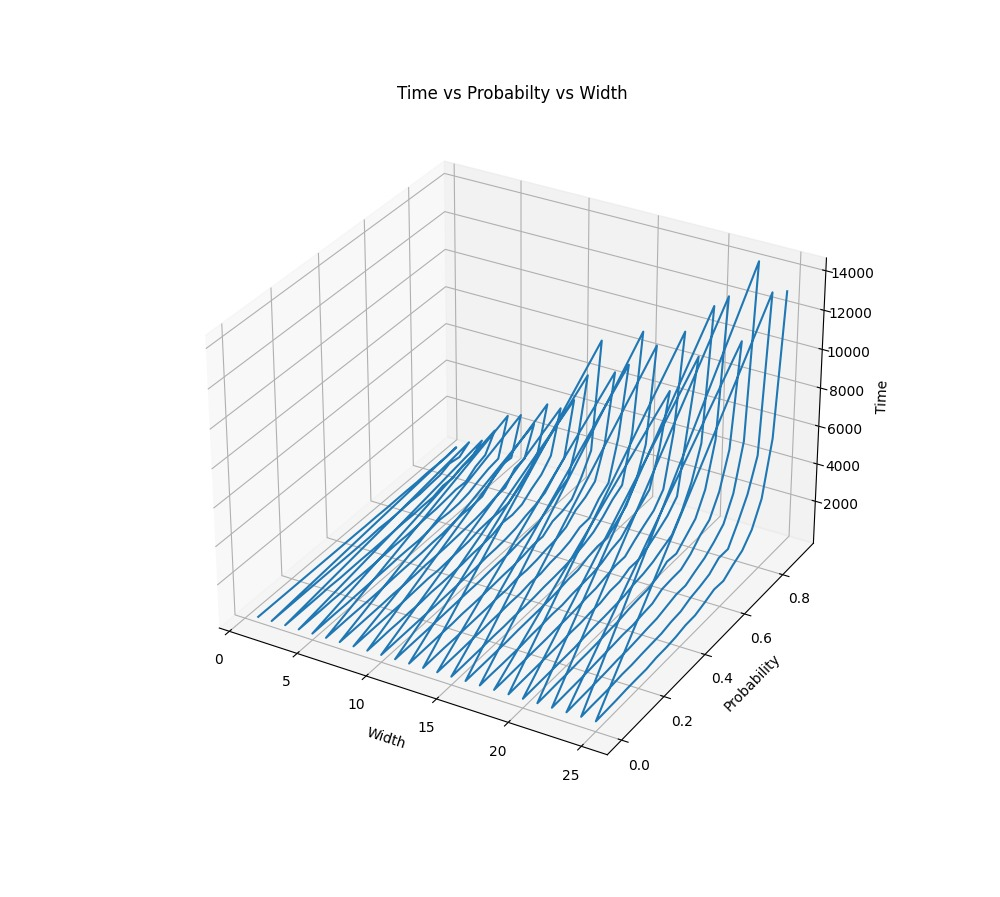
\includegraphics[scale = 0.81, width = 18.0 cm]{graph.jpg}
        \end{figure}

\end{document}